
% ------------------------------------------------------------------------------------------------------------------------------------------------
\chapter{System and design overview}
\label{chap:system-design}

The system, from here to be referred to by the name ,,\textit{Oculus}'', is designed with an asynchronous as well as distributed aproach in mind. In order to achieve high asynchrononisity between obtaining new reference data, and running jobs such as ,,\textit{compare video1 with the reference database}'', the system was split into two primary components: 

\begin{itemize}
  \item \textbf{loader} -- which is responsible for obtaining more and more reference material. It persists and initially processes the videos, as well as any related metadata. In a real system this reference data would be provided by partnering content providers, yet for this 
  \item \textbf{analyser} -- which is responsible for preparing and scheduling job pipelines for execution on top of the Hadoop cluster and reference databases.
\end{itemize}

To further illustrate the separate components and their interactions Figure \ref{fig:system-overview} shows the different interactions within the system.

\begin{figure}[hc!]
 \centering
  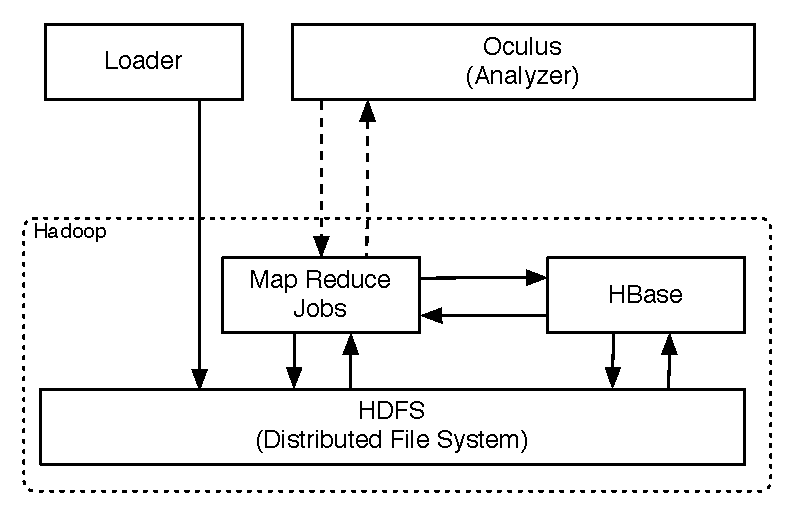
\includegraphics[scale=0.9]{./diagrams/high-level-system.pdf}
  \caption{High level overview of the system's architecture}
  \label{fig:system-overview}
\end{figure}

% ------------------------------------------------------------------------------------------------------------------------------------------------
\section{Loader}
The Loader component is responsible for obtaining as much as possible ,,reference data'', by which I mean video material -- from sites such as \textit{youtube.com} or video hosting sites. Please note that for the sake of this thesis (and legal safety) the downloaded content was limited to movie trailers (which are freely available on-line) as well as series opening, ending sequences.

While I will refer to the Loader (as a system) in singular, it should be noted that in fact there are multiple instances of it running in the cluster.
Thanks to the use of Akka's \cite{akka-docs} Actor Model abstractions (and \textit{remoting} module \cite{akka-remoting}), in which the physical location of an Actor plays is of no importance -- meaning, that the receiving Actor does not have to be on the same host as the sending Actor.

The system consists of 4 types of Actors each of which has multiple instances which are spread out on many nodes in the cluster.
Some tasks can only be sent to local Actors (any work requiring an already downloaded file), but messages related to crawling and initially downloading
the video material can be spread throughout the cluster. I will now briefly describe the different Actor roles that exist in the system and then explain the interactions between then on an example.

\begin{itemize}
  \item \textbf{YouTubeCrawlActor} -- is capable of fetching and YouTube websites and generate Messages triggering
                                    either further crawling of ,,related video sites'' (\verb|Crawl(siteId: String)|) or downloading of the 
                                    currently accessed video (by sending a \verb|Download(movieId)| message),
    \subitem  \textbf{receives:}
      \subsubitem 1 -- \verb|Crawl(siteId: String)| message
    \subitem  \textbf{sends:}
      \subsubitem 0 or n -- \verb|Crawl(siteId: String)| - where n is the number of ,,related video'' links found on the site. 
                                                           If crawling is turned off, no messages will be sent.

  \item \textbf{DownloadActor} -- is responsible for downloading the movie from youtube in it's original format (in the presence of many formats, 
                                the highest quality file will be downloaded). This Actor decides if a video is legal to download or not, because it also
                                obtains the movie's metadata -- only trailers and opening sequences of series are downloaded during for the sake of this 
                                thesis.
                                
  \item \textbf{ConversionActor} -- is responsible for converting the downloaded video material into raw frame data (bitmaps).
    \subitem  \textbf{receives:}
      \subsubitem \verb|Convert(localVideoFile: java.util.File)| -- This message must come from a local Actor, since the path refers to the local file system.
    \subitem  \textbf{sends:}
      \subsubitem \verb|Upload(framesDirectory: java.util.File)| -- when the finished converting to bitmaps, it will send and \verb|Upload| 
                                                                    message to one of the\verb|HDFSUploadActors|, pointing to the directory where the 
                                                                    output bitmaps have been written.
                                                                    
  \item \textbf{HDFSUploadActor} -- is responsible for optimally storing the sequence of bitmaps in Hadoop. This includes converting a series of 
                                  relatively small (around 2MB per frame) files into one Sequence File on HDFS. Sequence Files and the need for their use
                                  will be explained in detail in section \ref{sec:sequence-files}.
  \subitem \textbf{receives:}
    \subsubitem \verb|Upload(framesDirectory: java.util.File)| -- pointing to a local directory where the bitmap files have been stored.
                                                                 This message must come from a local actor, since the path refers to the local file system.
\end{itemize}

% -------------------------------------------------------------------------------------------------------------------------------------------------
\newpage
\subsection{Obtaining reference video material}
\label{sec:obtaining-reference-material}
In this subsection I will discuss the process of obtaining video material by the Loader subsystem, as well as explain which parts can be executed on different nodes of the cluster. The Figure \ref{fig:high-level-loader} should help in understanding the basic workflow.

\begin{figure}[ch!]
  \centering
  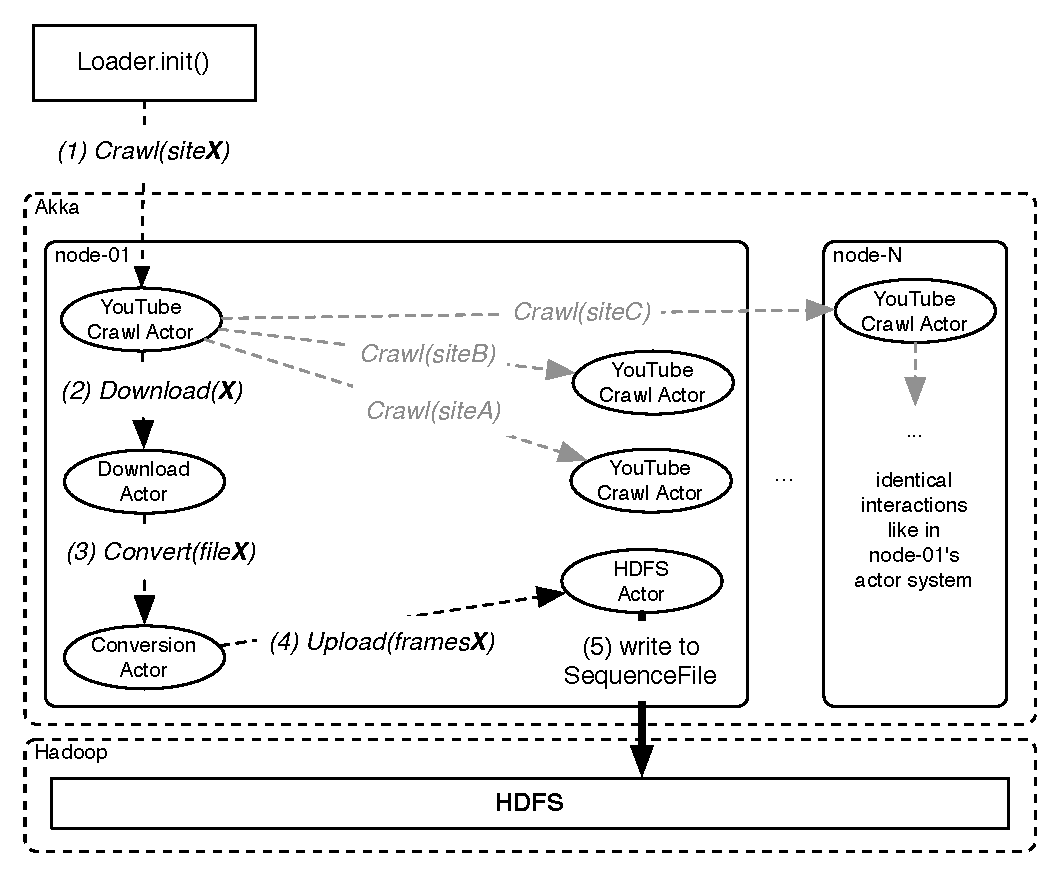
\includegraphics[scale=0.9]{./diagrams/loader-high-level.pdf}
  \caption{Overview of messages passed within the Loader's actor system. Greyed out messages are also sent, but are not on the critical path leading to obtaining material from \textit{siteX} into HDFS.}
  \label{fig:high-level-loader}
\end{figure}

\subsubsection{Step 1 - \textit{Crawl} messages}
The initiating message for each flow within the Loader is a \textit{Crawl(siteUrl)}, where siteUrl is a valid youtube video url.
The receiving YouTubeCrawlActor will react to such message by fetching and extracting the related video site urls and will forward those using the same kind of \textit{Crawl} messages. The second, yet most important, reaction is sending a \textit{Download(movieId)} message to an instance of an DownloadActor -- it  can reside on any node in the cluster, which allows us to spread the down-link utilisation between different nodes in the cluster.

It is worth pointing out that the receivers of these messages can be remote Actors, that is, can be located on a different node in the cluster than the sender. In order to guarantee spreading of the load among the many actors within the system (across nodes in the cluster), I am using a strategy called ,,Smallest Inbox Routing''. This technique uses a special ,,Router Actor'' which is responsible for a number of Routees (target Actors), and decides to deliver a message
only to the Actor who has the smallest amount of messages ,,not yet processed'' (which are kept in an Queue called the ,,Inbox'', hence the strategy's name).

\subsubsection{Step 2 - \textit{Download} messages}


\subsubsection{Step 3 - \textit{Convert} messages}
\subsubsection{Step 4 - \textit{Convert} messages}
\subsubsection{Step 4 - Writing the data to HDFS}

Since the reference data is fetched from youtube, implementing a crawler is fairly simple and requires only to fetch the site's HTML source and extract any ,,related'' video pages (which are contained on the right hand side on the youtube website). Using this the system will automatically continue fetching similar videos, for a few \textit{seed sites}. This is done by sending an initial message (1) via an asynchronous call to \verb|YouTubeCrawlActor|. It will fetch the page's sources, parse out all ,,related video'' urls and then send these to other \verb|YouTubeCrawlActor|s in the it's own local system or across the network, to another node in the cluster running another Actor System with the same types of Actors -- this remoting technique has many benefits which will be discussed in the subsection \ref{sec:location-transparency}.

% ------------------------------------------------------------------------------------------------------------------------------------------------
\section{Analyser}
\label{sec:analyser}
The analyser component is responsible for orchestrating Map Reduce jobs and submitting them to the cluster. Results of jobs are written to either HBase or plain TSV (\textit{Tab Separated Values}) Files. Figure \ref{fig:analyser-high-level} depicts the typical execution flow of an analysis process issued by Oculus.

\begin{figure}[ch!]
  \centering
  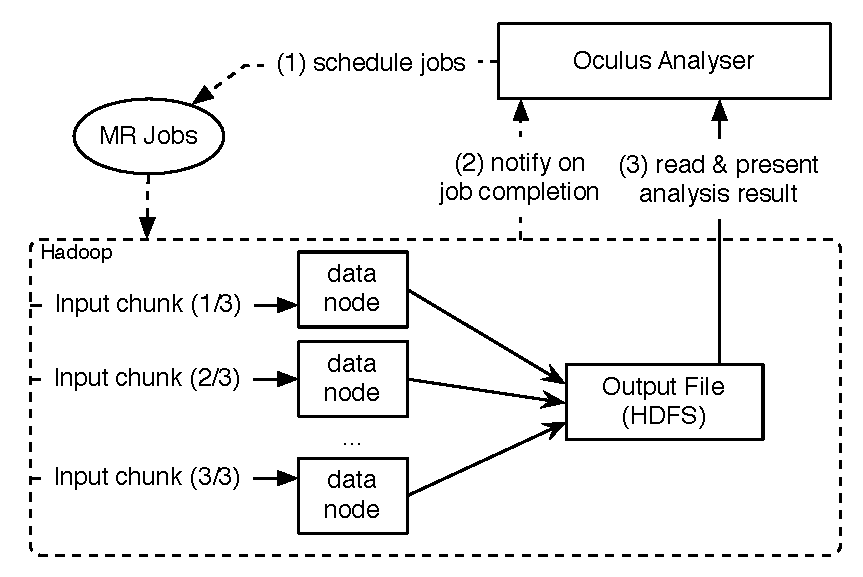
\includegraphics[scale=0.9]{diagrams/analyser-high-level.pdf}
  \caption{When storing a small file in HDFS, it still takes up an entire block. The grey space is not wasted on disk, but causes the \textit{name-node} memory problems.}
  \label{fig:analyser-high-level}
\end{figure}

In step 1 the \textit{job pipeline} is being prepared by the program by aggregating required metadata and preparing the job pipeline, which often consists of more than just one Map Reduce job -- in fact, most analysis jobs performed by Oculus require at least 3 or more Map Reduce jobs to be issued to the cluster. It is important to note that some of these jobs may be dependent on another task's output and this cannot be run in parallel. On the other hand, if a job requires calculating all histograms for all frames of a movie as well as calculating something different for each of these frames -- these jobs can be executed in parallel and will benefit from the large number of data nodes which can execute these jobs.

The 2nd step on Figure \ref{fig:analyser-high-level} is important because Oculus may react with launching another analysis job based on the notification that one pipeline has completed. This allows to keep different pipelines separate, and trigger them reactively when for example all it's dependencies have been computed in another pipeline.

For most applications though the 3rd step in a typical Oculus Job would be to read and present top N results to the issuer of the job, which for a question like ,,Which movie is similar to this one?'' would be the top N most similar movies (their names, identifiers as well as match percentage).

% ------------------------------------------------------------------------------------------------------------------------------------------------
\subsection{Frame-by-frame data and the HDFS ,,small--files problem''}
\label{sec:sequence-files}
Most algorithms used in Oculus operate on a frame-by-frame basis, which means that it is most natural to store all data as ,,data for frame 343 from movie XYZ''.
This applies to everything from plain bitmap data of a frame to metrics such as histograms of colours of a given frame or other metadata like the extracted text content found in this frame.

Sadly this abstraction does not work nicely with Hadoop, it would cause the well--known ,,small-files problem'' which leads to \textit{major} performance degradation of the Hadoop cluster is left undressed. In this section I will focus on explaining the problem and what steps have been taken to prevent it from manifesting in the presence of millions of ,,by-frame'' data points.

Hadoop uses so called ,,blocks'' as smallest atomic unit that can be used to move data between the cluster.
The default block size is set to \textit{64 megabytes} on most Hadoop distributions (including vanilla Apache Hadoop which this implementation is using).

This also means that if the DFS takes a write of one file (assuming the \textit{replication factor} equals 1) it will use up one block.
By itself this is not worrisome, because other than in traditional (local) file systems such as EXT3 for example, when we store N bytes in a block on HDFS,
the the file system can still use block's unused space. Figure \ref{fig:no-sequence-file} shows the structure of a block storing only one frame of a movie.

\begin{figure}[ch!]
  \centering
  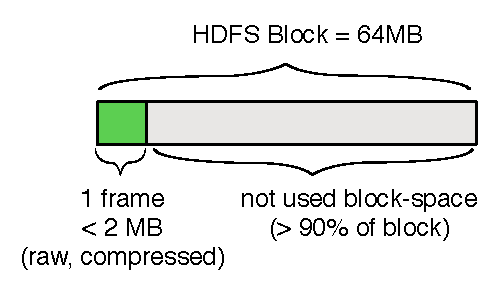
\includegraphics[scale=0.9]{diagrams/no-sequence-file.pdf}
  \caption{When storing a small file in HDFS, it still takes up an entire block. The grey space is not wasted on disk, but causes the \textit{name-node} memory problems.}
  \label{fig:no-sequence-file}
\end{figure}

The problem stemming from writing small files manifests not directly by impacting the used disk space, but in increasing memory usage in the clusters so called \textit{name-node}. The name-node is responsible for acting as a lookup table for locating the blocks in the cluster. Since name-node has to keep 150KB of metadata for each block in the cluster, creating more blocks than we actually need quickly forces the name-node to use so much memory, that it may run into long garbage collection pauses, degrading the entire cluster's performance. To put precise numbers to this -- if we would be able to store 500MB of data in an optimal way, storing them on HDFS would use 8 blocks -- causing the name node to use approximately 1KB of metadata. On the other hand, storing this data in chunks of 2MB (for example by storing each frame of a movie, uncompressed) would use up 250 HDFS blocks, which results in additional 36KB of memory used on the name-node, which is 4.5 times as much (28KB more) as with optimally storing the data! Since we are talking about hundreds of thousands of files, such waste causes a tremendous unneeded load on the name-node.

It should be also noted, that when running map-reduce jobs, Hadoop will by default start one map task for each block it's processing in the given Job. Spinning up a task is an expensive process, so this too is a cause for performance degradation, since having small files causes more \textit{Map tasks} being issued for the same amount of actual data Hadoop will spend more time waiting for tasks to finish starting and collecting data from them than it would have to.

% ------------------------------------------------------------------------------------------------------------------------------------------------
\subsubsection{Defining Map Reduce Pipelines using Scalding and Cascading}
The primary language used for implementing all Oculus jobs, including Map Reduce jobs is Scala \cite{scala}

\begin{lstlisting}[caption={Simplest Scalding job used in Oculus -- each frame perceptual hashing}, label={lst:simplest-scalding-job}]

\end{lstlisting}



% ------------------------------------------------------------------------------------------------------------------------------------------------
\subsubsection{Sequence Files}
\label{sequence-file}
The solution applied in the implemented system to resolve the small files problem is based on a technique called ,,Sequence Files'', which are a manually controlled layer of abstraction on top of HDFS blocks. There are multiple Sequence file formats accepted by the common utilities that Hadoop provides \cite{hadoop-seq-files} but they all are \textit{binary header-prefixed key-value formats}, as visualised Figure \ref{fig:sequence-file}.


\begin{figure}[ch!]
  \centering
  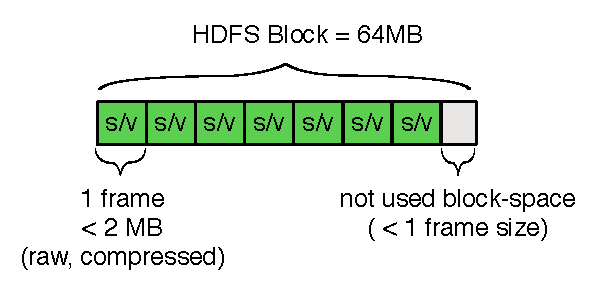
\includegraphics[scale=0.9]{diagrams/sequence-file.pdf}
  \caption{A SequenceFile allows storing of multiple small chunks of data in one HDFS Block.}
  \label{fig:sequence-file}
\end{figure}

Using Sequence Files resolves all previously described problems related to small files on top of HDFS. Files are no longer ,,small'', at least in Hadoop's perception,
since access of frames of a movie is most often bound to access other frames of this movie we don't suffer any drawbacks from such storage format.

Another solution that could have been applied here is the use of HBase and it's key-value design instead of the explicit use of Sequence Files, yet this would not yield much performance nor storage benefits as HBase stores it's Table data in a very similar format as Sequence Files. The one benefit from using HBase in order to avoid the small files problem would have been random access to any frame, not to ,,frames of this movie'', but since I don't have such access patterns and it would complicate the design of the system I decided to use Sequence Files instead.






